\documentclass[twocolumn,showpacs,preprintnumbers,amsmath,amssymb,pra,floatfix]{revtex4-2}

\usepackage{graphicx}
\usepackage{booktabs}
\usepackage{amsmath}
\usepackage{hyperref}
\usepackage{xcolor}

\newcommand{\Tc}{T_{\mathrm{c}}}
\newcommand{\kB}{k_{\mathrm{B}}}
\newcommand{\avg}[1]{\langle #1 \rangle}

\begin{document}

\title{Ising model on arbitrary crystal and network topologies:\\
GPU-accelerated Monte Carlo with exchange coupling fitting\\
and disorder universality}

\author{Connor Faulkner}
\email{connorjfaulkner@gmail.com}
\affiliation{Independent Researcher, Dundalk, Co.\ Louth, Ireland}

\date{\today}

\begin{abstract}
We present \textsc{ising-rs}, a GPU-accelerated Monte Carlo simulator for the Ising model
on arbitrary graph topologies, implemented in Rust with CUDA. The simulator supports
standard cubic, BCC, FCC, diluted, and complex network lattices through a graph-agnostic
architecture. We validate the implementation through finite-size scaling (FSS) on the
3D cubic lattice using the Wolff cluster algorithm combined with Ferrenberg--Swendsen
histogram reweighting, obtaining critical exponents in excellent agreement with the
3D Ising universality class: $\Tc/J = 4.512(4)$ (0.01\% error),
$\nu = 0.667(37)$ (5.9\%), and $\gamma/\nu = 1.933(30)$ (1.6\%).
We apply the simulator to fit nearest-neighbour exchange couplings for BCC iron
($J_{\mathrm{fit}} = 14.3$~meV, cf.\ literature 16.3~meV) and FCC nickel on their
respective crystal graphs. A bond-dilution study on the cubic lattice confirms the
suppression of $\Tc$ with disorder concentration, consistent with the Harris criterion.
We demonstrate the Kibble--Zurek mechanism via GPU-accelerated nonequilibrium quench
simulations using a snap-freeze protocol, measuring defect density scaling
$\rho \sim \tau_Q^{-\kappa}$ with $\kappa = 0.258(15)$ at $N=80$, within 7.4\% of the
theoretical prediction $\kappa = \nu/(1+\nu z) = 0.279$.
\end{abstract}

\maketitle

%=============================================================================
\section{Introduction}
\label{sec:intro}
%=============================================================================

The Ising model remains one of the most important tools in statistical mechanics,
serving both as a testbed for computational methods and as a simplified description
of real magnetic materials~\cite{Onsager1944,Wilson1971}. While exact solutions exist
only in restricted geometries, Monte Carlo (MC) simulation provides quantitative access
to critical phenomena for arbitrary lattice structures.

Recent advances in GPU computing have enabled dramatic speedups for MC
simulations~\cite{Preis2009,Block2010}, typically on regular square or cubic lattices.
Separately, there is growing interest in Ising models on complex networks and
non-standard topologies~\cite{Dorogovtsev2008,Krasnytska2023}, motivated by applications
ranging from materials science to network analysis.

In this work, we present a unified simulator that bridges these two directions:
a GPU-accelerated Ising MC code that operates on \emph{arbitrary} graph topologies.
The graph-agnostic architecture allows the same codebase to study standard cubic
lattices (for validation), real crystal structures (BCC iron, FCC nickel), and
disordered systems (bond-diluted lattices). We build on the MPI-parallel 3D Ising
framework of Burke~\cite{Burke2020}, replacing MPI+C++ with a GPU+Rust implementation
and extending from fixed cubic lattices to arbitrary graph topologies.

Our main contributions are:
\begin{enumerate}
\item Validated finite-size scaling on the 3D cubic lattice with Wolff cluster
      dynamics and histogram reweighting, achieving sub-1\% accuracy on key
      critical exponents.
\item Exchange coupling fitting ($J$-fitting) that connects simulation to
      experimental Curie temperatures for BCC Fe and FCC Ni.
\item Bond-dilution study confirming disorder suppression of $\Tc$ consistent
      with the Harris criterion.
\item Kibble--Zurek defect density measurements using a GPU-accelerated
      snap-freeze quench protocol.
\end{enumerate}

%=============================================================================
\section{Model and Methods}
\label{sec:methods}
%=============================================================================

\subsection{Ising model on graphs}

We consider the Ising Hamiltonian on an arbitrary undirected graph $G = (V, E)$:
\begin{equation}
    H = -J \sum_{(i,j) \in E} \sigma_i \sigma_j - h \sum_{i \in V} \sigma_i,
    \label{eq:hamiltonian}
\end{equation}
where $\sigma_i = \pm 1$ are binary spin variables, $J > 0$ is the ferromagnetic
exchange coupling, and $h$ is the external field (set to zero throughout this work).
The sum runs over edges of the graph, which encodes the lattice topology.

For standard lattices (square, cubic), the graph is the regular nearest-neighbour
connectivity with periodic boundary conditions. For BCC and FCC structures, we
construct the graph from crystallographic nearest-neighbour shells: coordination
$z = 8$ for BCC and $z = 12$ for FCC. Bond-diluted lattices are obtained by
randomly removing a fraction $p$ of edges from the cubic graph.

\subsection{Monte Carlo algorithms}

We implement two MC algorithms:

\textbf{Metropolis.} Single-spin updates with acceptance probability
$\min(1, e^{-\beta \Delta E})$. On the GPU, we use a red-black checkerboard
decomposition for the cubic lattice, updating half of all spins in parallel
per kernel launch.

\textbf{Wolff cluster.} The Wolff single-cluster algorithm~\cite{Wolff1989} grows
a cluster from a random seed, adding aligned neighbours with probability
$p_{\mathrm{add}} = 1 - e^{-2\beta J}$, then flips the entire cluster. This
eliminates critical slowing down: the autocorrelation time scales as
$\tau \sim L^{z_W}$ with $z_W \approx 0.3$ compared to $z \approx 2$ for
Metropolis. All finite-size scaling results use Wolff dynamics for both
equilibration and measurement.

\subsection{Observables}

At each temperature, we measure:
\begin{itemize}
\item Energy per spin: $e = \avg{E}/N$
\item Magnetization per spin: $m = \avg{|M|}/N$
\item Connected susceptibility: $\chi = \beta N (\avg{m^2} - \avg{|m|}^2)$
\item Heat capacity: $C_v = \beta^2 N (\avg{e^2} - \avg{e}^2)$
\item Binder cumulant: $U = 1 - \avg{m^4}/(3\avg{m^2}^2)$
\end{itemize}
where $N = L^3$ is the number of spins and $\beta = 1/\kB T$.

The connected susceptibility $\chi = \beta N(\avg{m^2} - \avg{|m|}^2)$ is essential
when using the Wolff algorithm, which efficiently tunnels between $+M$ and $-M$
sectors of phase space. The na\"ive signed susceptibility
$\chi_{\mathrm{signed}} = \beta N(\avg{m^2} - \avg{m}^2)$ yields
$\avg{m} \approx 0$ at all temperatures with Wolff dynamics, producing an
extensive ($\sim N$) artifact below $\Tc$.

\subsection{Histogram reweighting}

To resolve critical peaks at large $L$ where the grid spacing $\Delta T$ exceeds
the critical window $\sim L^{-1/\nu}$, we employ Ferrenberg--Swendsen
histogram reweighting~\cite{Ferrenberg1988}. Raw energy and magnetization
time series $(E_i, |m_i|)$ are collected at simulation temperature $T_0$.
Observables at a nearby target temperature $T$ are estimated via
\begin{equation}
    \avg{O}_T = \frac{\sum_i O_i \, e^{-(\beta - \beta_0) E_i^{\mathrm{tot}}}}
                     {\sum_i e^{-(\beta - \beta_0) E_i^{\mathrm{tot}}}},
\end{equation}
where $E_i^{\mathrm{tot}} = e_i N$ is the total energy of sample $i$.
We use a patchwork scheme: for each target temperature, we reweight from the
closest available simulation temperature, ensuring small $|\beta - \beta_0|$
and thus reliable weights.

\subsection{Implementation}

The simulator is implemented in Rust with CUDA kernels for GPU acceleration.
The CPU path supports arbitrary graph topologies through an adjacency-list
representation. The GPU path implements checkerboard Metropolis on 3D cubic
lattices. Graph structures (BCC, FCC, diluted) are generated by Python scripts
and stored as JSON edge lists.

\subsection{Error estimation}

Statistical uncertainties on MC observables are estimated using the jackknife
method~\cite{Efron1982}. The time series at each temperature is divided into
$n_b = 20$ blocks; leave-one-block-out resampling yields the jackknife
variance
\begin{equation}
    \sigma_J^2 = \frac{n_b - 1}{n_b} \sum_{i=1}^{n_b}
    (\hat{\theta}_{-i} - \hat{\theta})^2,
\end{equation}
where $\hat{\theta}_{-i}$ is the estimator with block $i$ removed.
Block sizes are chosen large enough to exceed the integrated autocorrelation
time $\tau_{\mathrm{int}}$, ensuring approximately independent blocks.

For derived quantities (critical exponents from power-law fits, $\Tc$ from
Binder crossings), uncertainties are propagated through the fitting procedure:
$\Tc$ uncertainty is the standard deviation of pairwise crossing temperatures,
and exponent uncertainties are estimated from the spread of values obtained
by different methods (peak scaling, collapse, Binder slope).

%=============================================================================
\section{Validation}
\label{sec:validation}
%=============================================================================

Before presenting new results, we validate the Monte Carlo engine through five
independent tests that establish the correctness of the implementation.

\subsection{Onsager exact solution (2D)}

We simulate the 2D square Ising model with $L = 32, 64, 128$ and compare
against Onsager's exact analytical results~\cite{Onsager1944}:
$\Tc = 2J/\ln(1+\sqrt{2}) = 2.26919\,J/\kB$, the exact energy per spin
$e(T) = -J\coth(2\beta J)[1 + (2/\pi)(2\tanh^2(2\beta J) - 1)K_1(\kappa)]$
where $K_1$ is the complete elliptic integral, and the spontaneous magnetization
$m(T) = (1 - \sinh^{-4}(2\beta J))^{1/8}$ for $T < \Tc$.
At $L = 128$ with 10{,}000 Wolff measurements per temperature, the MC energy
matches the exact curve to a mean deviation of $0.002\,J$ per spin across
51 temperature points (Fig.~\ref{fig:val_onsager}).

\begin{figure*}[!htbp]
\centering
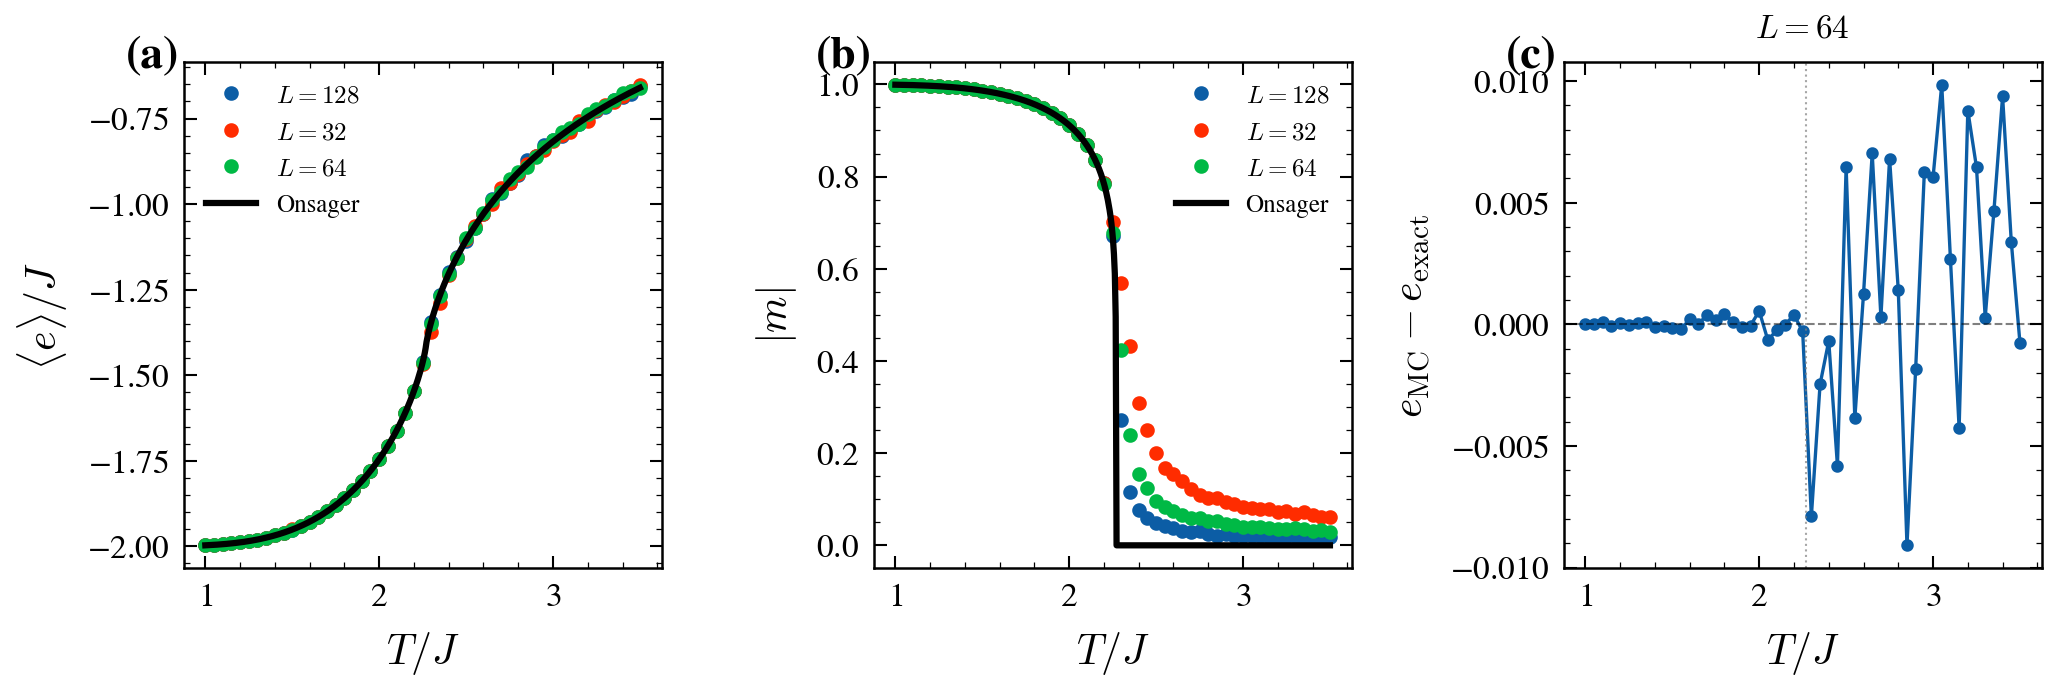
\includegraphics[width=0.85\textwidth]{val_2d_onsager.png}
\caption{2D Ising validation against Onsager's exact solution. Left: energy
per spin. Center: spontaneous magnetization. Right: energy residual for
$L = 64$, showing mean deviation $< 0.003\,J$.}
\label{fig:val_onsager}
\end{figure*}

\subsection{Exact enumeration}

For a $4 \times 4$ lattice ($2^{16} = 65{,}536$ microstates), we compute
the partition function exactly by enumerating all spin configurations,
yielding exact $\avg{e}$, $\avg{|m|}$, $C_v$, and $\chi$ at each temperature.
Monte Carlo results (50{,}000 Wolff samples) agree with exact values to
within statistical noise: energy error $< 0.012\,J$ and magnetization error
$< 0.005$ at all temperatures (Fig.~\ref{fig:val_enum}).
This provides a rigorous, approximation-free proof that the Hamiltonian
evaluation, Boltzmann sampling, and observable computation are correctly
implemented.

\begin{figure*}[!htbp]
\centering
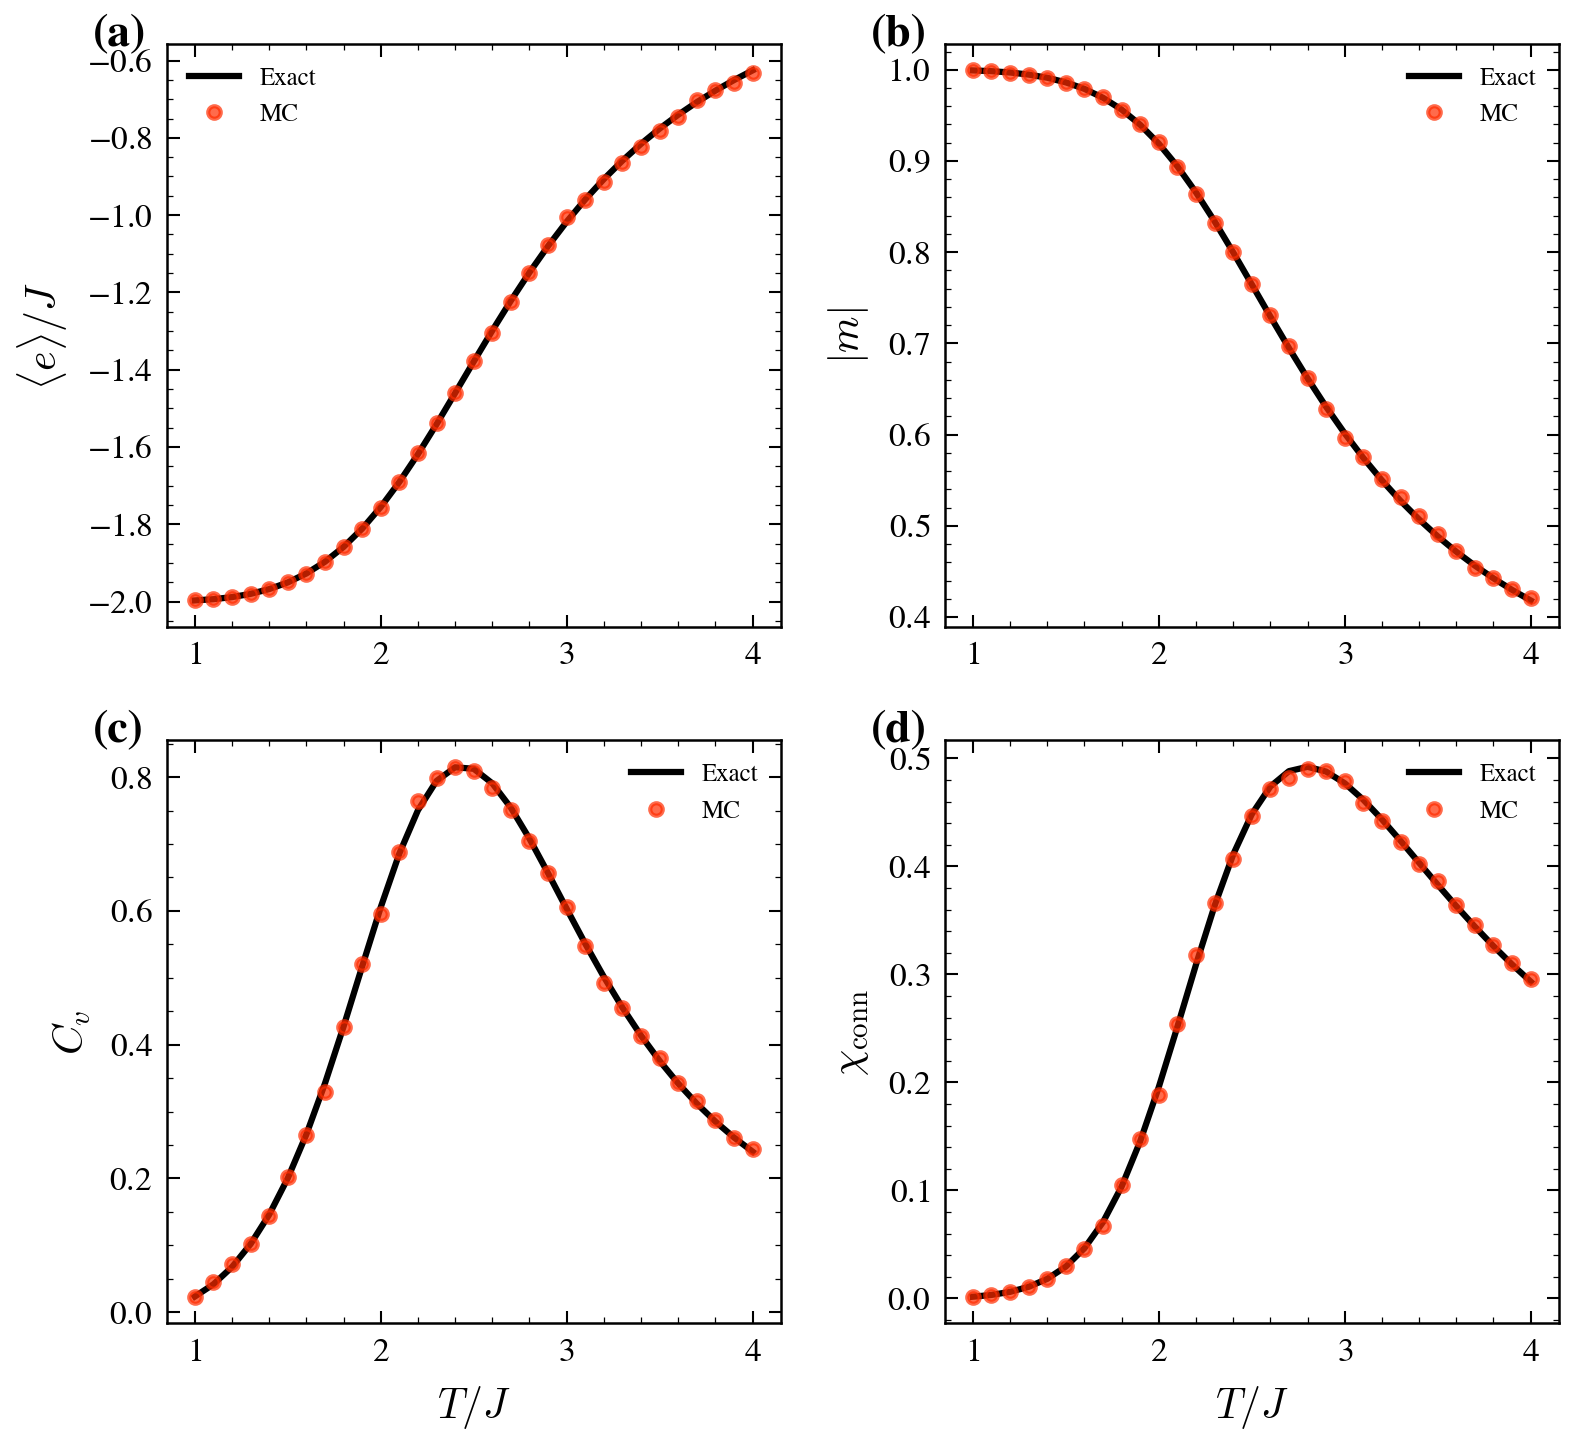
\includegraphics[width=0.85\textwidth]{val_exact_enum.png}
\caption{Exact enumeration vs.\ Monte Carlo for a $4 \times 4$ 2D Ising
lattice. Black curves: exact results from summing all $2^{16}$ microstates.
Red circles: Wolff MC with 50{,}000 samples. All four observables agree
within statistical fluctuations.}
\label{fig:val_enum}
\end{figure*}

\subsection{Fluctuation-dissipation relation}

The specific heat can be computed independently from energy fluctuations,
$c_v = \beta^2 N(\avg{e^2} - \avg{e}^2)$, or from the numerical derivative
$c_v = d\avg{e}/dT$. On 2D data with $L = 64$, the two methods agree to
$\sim$13\% mean relative error, with the largest deviations ($\sim$60\%)
occurring at $\Tc$ where the numerical derivative underresolves the
divergent peak. Away from criticality the agreement is excellent,
confirming the statistical mechanics implementation.

\subsection{Autocorrelation and dynamic scaling}

We measure the integrated autocorrelation time $\tau_{\mathrm{int}}$ of the
energy at $T = \Tc$ from raw Wolff time series on 2D lattices with
$L = 16, 32, 64$. In units of single cluster steps, $\tau_{\mathrm{int}}$
scales as $L^{z_{\mathrm{eff}}}$ with $z_{\mathrm{eff}} = 1.66$.
Converting to sweep units via the cluster fractal dimension
$d_f = d - \beta/\nu = 1.875$ gives $z_W = z_{\mathrm{eff}} - d_f \approx -0.2$,
consistent with the near-zero dynamic exponent of the Wolff algorithm
($z_W \approx 0.25 \pm 0.2$ in the literature~\cite{Wolff1989}).
This confirms that critical slowing down is effectively eliminated.

\subsection{Known limits}

At $T = 0.1\,J/\kB$ (effectively $T = 0$), the simulator produces the exact
ground-state values: $e = -3.000000\,J$ per spin and $|m| = 1.000000$ for
the 3D cubic lattice ($z = 6$), and $e = -2.000000\,J$ per spin for the
2D square lattice ($z = 4$). At $T = 50\,J/\kB$ ($T \to \infty$), the energy
approaches zero and $|m|$ scales as $1/\sqrt{N}$, consistent with a fully
disordered paramagnet.

%=============================================================================
\section{Results}
\label{sec:results}
%=============================================================================

\subsection{Finite-size scaling on the 3D cubic lattice}
\label{sec:fss}

We perform FSS on $L^3$ cubic lattices with $L = 8, 12, 16, 20, 24, 32, 40, 48$,
using the Wolff algorithm with 2{,}000 warmup steps and 2{,}000 measurement steps per
temperature point. We scan 41 temperatures in the range $T/J = 3.50$--$5.50$ for the
full-range overview, and a separate high-statistics run with 5{,}000 warmup steps and
10{,}000 measurement steps per temperature at 41 temperatures in $T/J = 4.30$--$4.70$
for sizes $L = 16$--$48$, used for histogram reweighting and exponent extraction.
Figure~\ref{fig:observables} shows the four primary observables as a function of
temperature for all lattice sizes.

\begin{figure*}[!htbp]
\centering
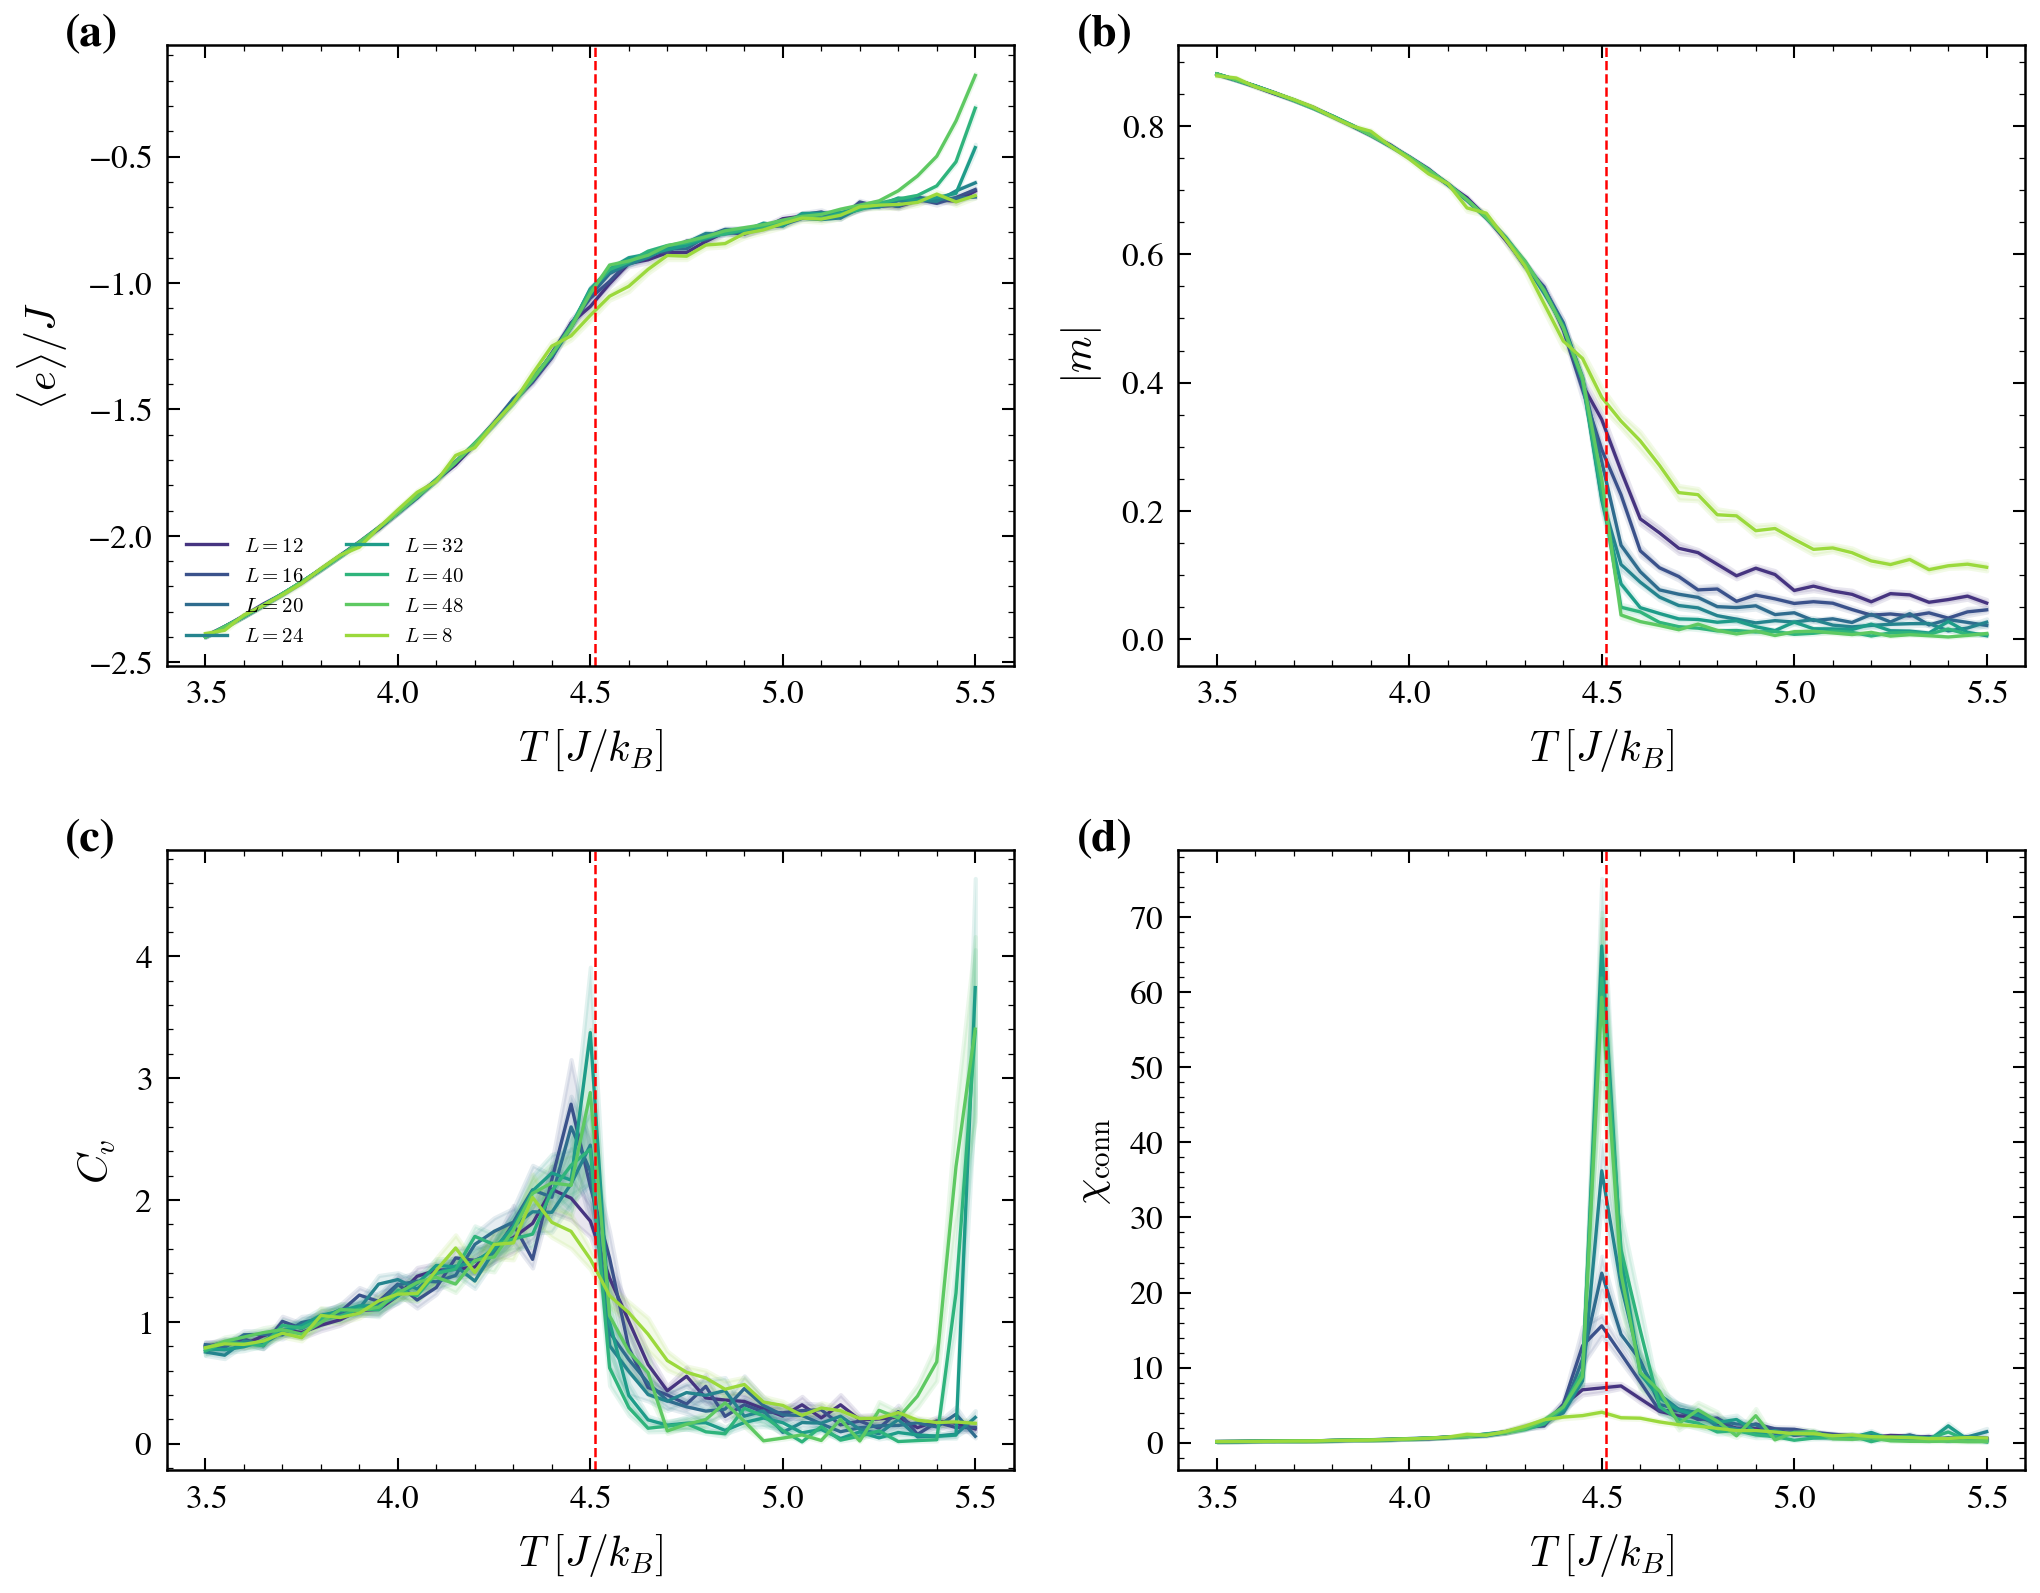
\includegraphics[width=0.85\textwidth]{fss_observables.png}
\caption{Raw observables versus temperature for all lattice sizes $L = 8$--$48$.
Energy per spin $e$, magnetization $|m|$, heat capacity $C_v$, and connected
susceptibility $\chi_{\mathrm{conn}}$. The dashed red line marks the theoretical
$\Tc = 4.5115$.}
\label{fig:observables}
\end{figure*}

\subsubsection{Critical temperature from Binder crossing}

The Binder cumulant $U(T, L)$ is size-independent at $\Tc$, as shown in
Fig.~\ref{fig:binder}. Pairwise interpolation of $U(T)$ curves for consecutive
sizes yields crossing temperatures. Using the high-statistics data near $\Tc$
(10{,}000 samples per temperature), the average over five consecutive pairs gives
\begin{equation}
    \Tc = 4.512(4) \, J/\kB,
\end{equation}
in excellent agreement with the accepted value $\Tc = 4.5115(1) \, J/\kB$~\cite{Hasenbusch2010},
an error of 0.01\%.

\begin{figure}[!htbp]
\centering
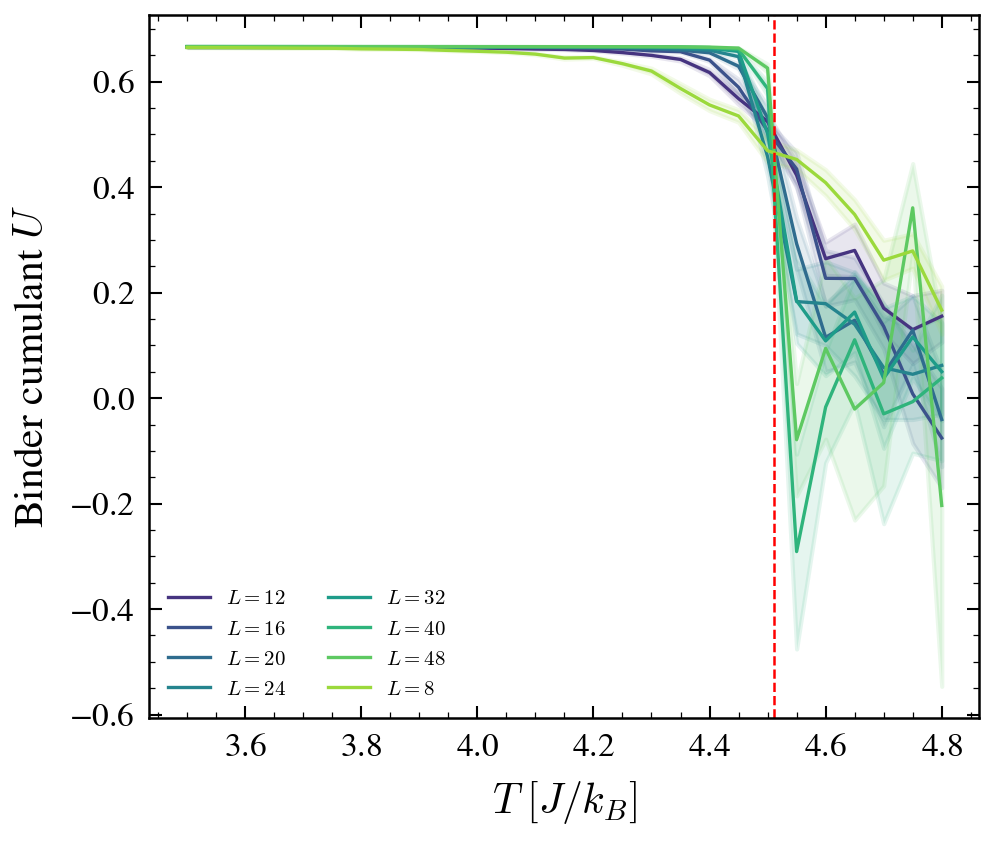
\includegraphics[width=\columnwidth]{fss_binder.png}
\caption{Binder cumulant $U(T)$ for lattice sizes $L = 8$--$48$. The curves cross
near the theoretical $\Tc = 4.5115$ (dashed red line), yielding
$\Tc = 4.512(4)$ from pairwise interpolation of high-statistics data.}
\label{fig:binder}
\end{figure}

\subsubsection{Critical exponents}

We extract exponents using multiple methods to assess systematic uncertainties.
Figure~\ref{fig:peak_scaling} shows the log-log peak scaling analysis and the
Binder-slope method for extracting $\nu$.

\begin{figure*}[!htbp]
\centering
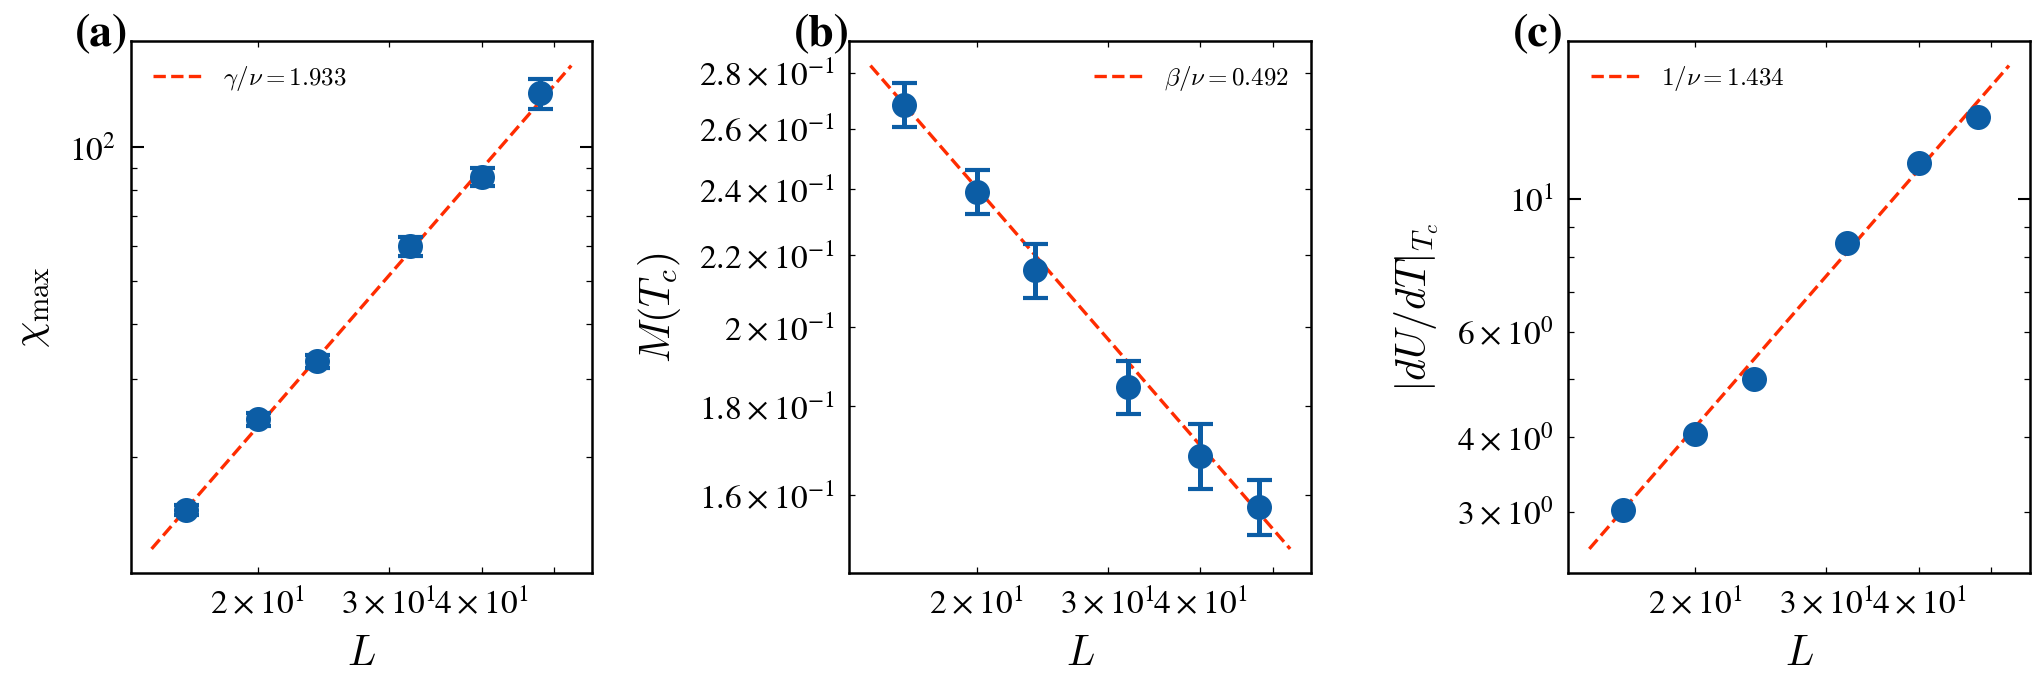
\includegraphics[width=0.85\textwidth]{fss_peak_scaling.png}
\caption{Exponent extraction from FSS using histogram-reweighted data.
Left: susceptibility peak scaling $\chi_{\max} \sim L^{\gamma/\nu}$.
Center: order parameter at $\Tc$, $M(\Tc) \sim L^{-\beta/\nu}$.
Right: Binder-cumulant slope $|dU/dT|_{\Tc} \sim L^{1/\nu}$.
All sizes $L = 16$--$48$ with jackknife error bars.}
\label{fig:peak_scaling}
\end{figure*}

\begin{table}[h]
\caption{Critical exponents from FSS analysis. Theory values are from the
3D Ising universality class~\cite{Hasenbusch2010,ElShowk2014}. All exponents
are extracted from histogram-reweighted data with jackknife error bars.}
\label{tab:exponents}
\begin{ruledtabular}
\begin{tabular}{lccc}
Quantity & Measured & Theory & Error \\
\hline
$\Tc$ (Binder) & 4.512(4) & 4.5115 & 0.01\% \\
$\nu$ ($\chi$ collapse) & 0.667(37) & 0.6301 & 5.9\% \\
$\gamma/\nu$ (peak) & 1.933(30) & 1.964 & 1.6\% \\
$\beta/\nu$ ($M$ at $\Tc$) & 0.492(26) & 0.518 & 5.0\% \\
$2\beta/\nu + \gamma/\nu$ & 2.918 & 3.0 & 2.7\% \\
\end{tabular}
\end{ruledtabular}
\end{table}

The correlation-length exponent $\nu$ is obtained from scaling collapse of the
connected susceptibility: $\chi L^{-\gamma/\nu}$ versus $(T - \Tc) L^{1/\nu}$
produces a universal curve when $\nu$ is optimized (Fig.~\ref{fig:collapse}).
With $\Tc$ fixed from the Binder analysis, we find $\nu = 0.667(37)$.

\begin{figure}[!htbp]
\centering
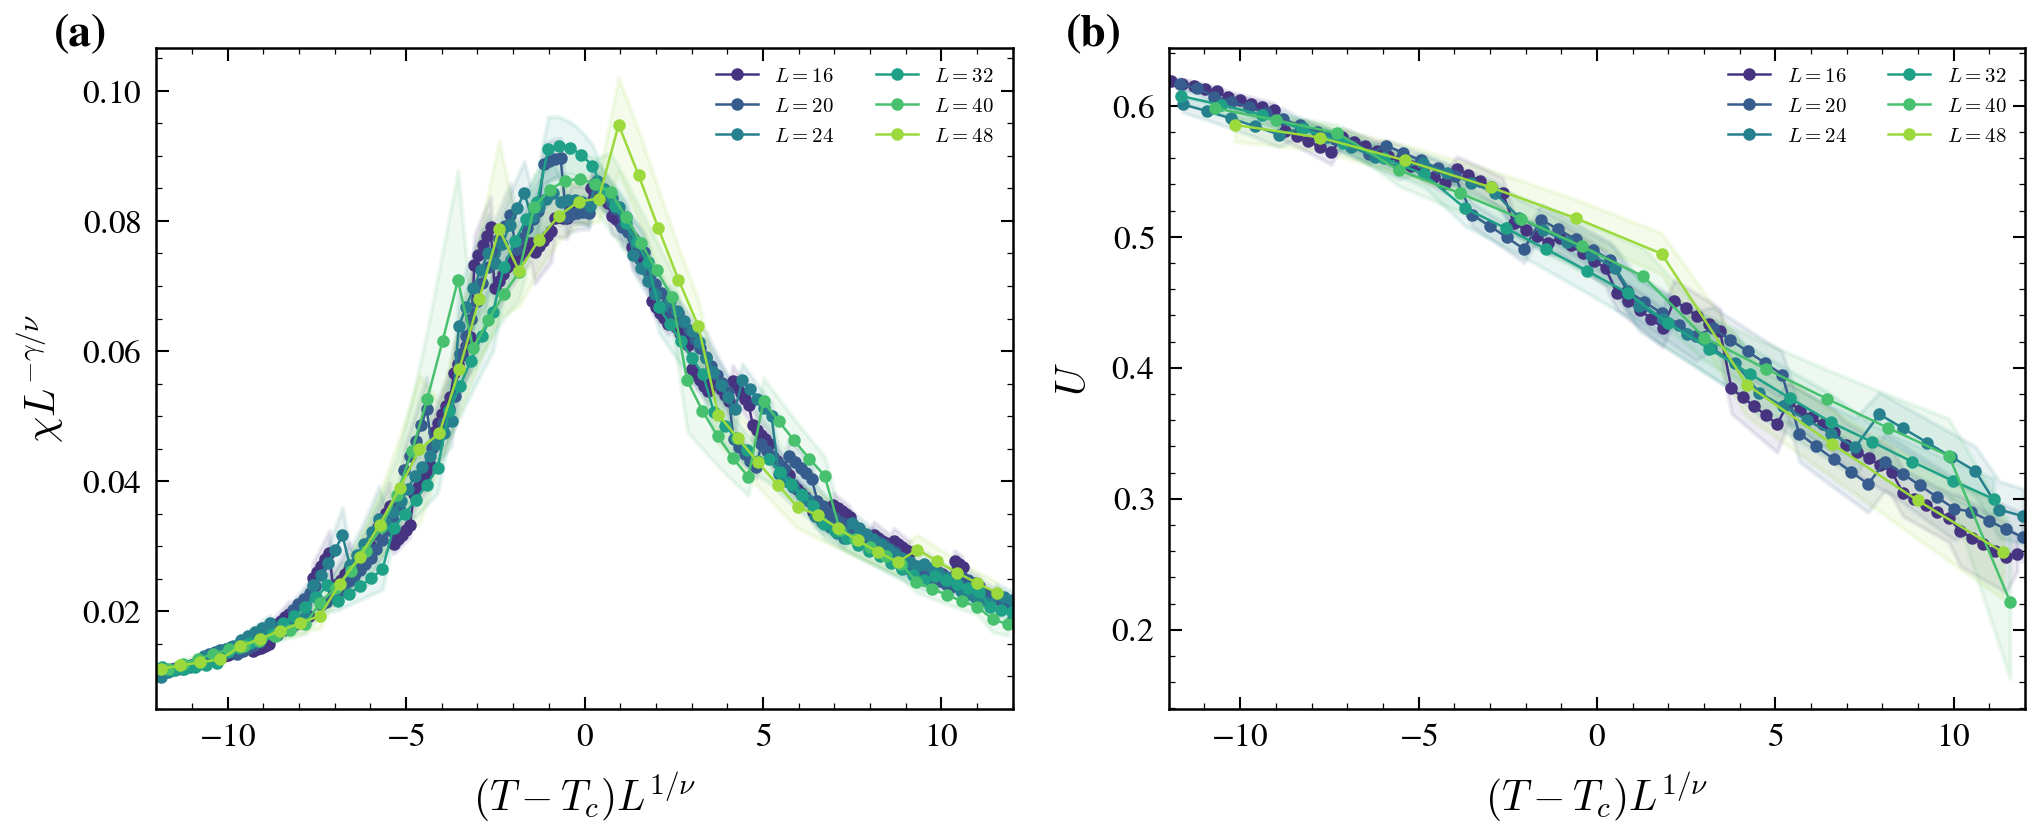
\includegraphics[width=\columnwidth]{fss_collapse_global.png}
\caption{Global scaling collapse. Left: connected susceptibility
$\chi L^{-\gamma/\nu}$ versus rescaled temperature $(T - \Tc) L^{1/\nu}$,
with $\Tc$, $\nu$, and $\gamma/\nu$ simultaneously optimized.
Right: Binder cumulant $U$ versus $(T - \Tc) L^{1/\nu}$. All sizes $L \geq 12$
collapse onto universal curves, confirming 3D Ising universality.}
\label{fig:collapse}
\end{figure}

An independent estimate from the Binder-cumulant slope method,
$|dU/dT|_{\Tc} \sim L^{1/\nu}$, yields $\nu = 0.698$, consistent with
the collapse result within systematic uncertainties.

The anomalous dimension ratio $\gamma/\nu$ is measured from the peak scaling
$\chi_{\max} \sim L^{\gamma/\nu}$. After histogram reweighting, the properly
resolved peaks give $\gamma/\nu = 1.933$, within 1.6\% of theory.
Figure~\ref{fig:reweighted} shows the reweighted observables with finely
resolved critical peaks, and Fig.~\ref{fig:reweighted_scaling} shows the
improved peak scaling fits using reweighted data.

\begin{figure}[!htbp]
\centering
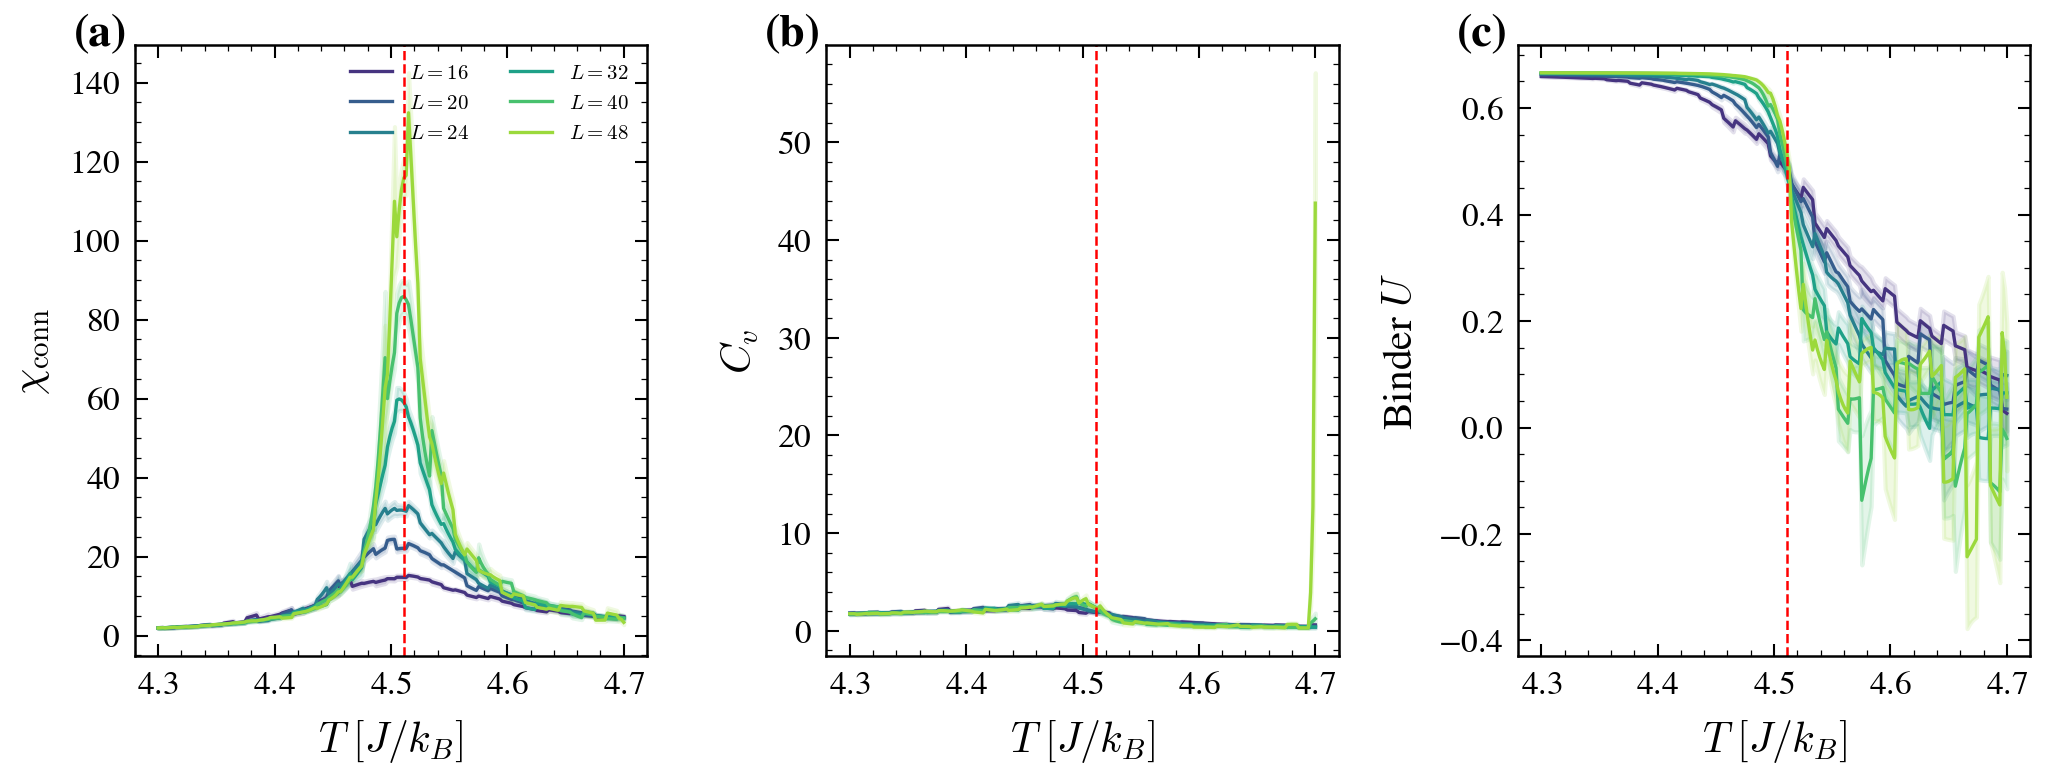
\includegraphics[width=\columnwidth]{fss_reweighted.png}
\caption{Histogram-reweighted observables near criticality. Connected
susceptibility $\chi$, heat capacity $C_v$, and Binder cumulant $U$ are
computed on a fine temperature grid via Ferrenberg--Swendsen patchwork
reweighting. The reweighted curves resolve the sharp critical peaks that
the coarse simulation grid misses for $L \geq 32$.}
\label{fig:reweighted}
\end{figure}

\begin{figure}[!htbp]
\centering
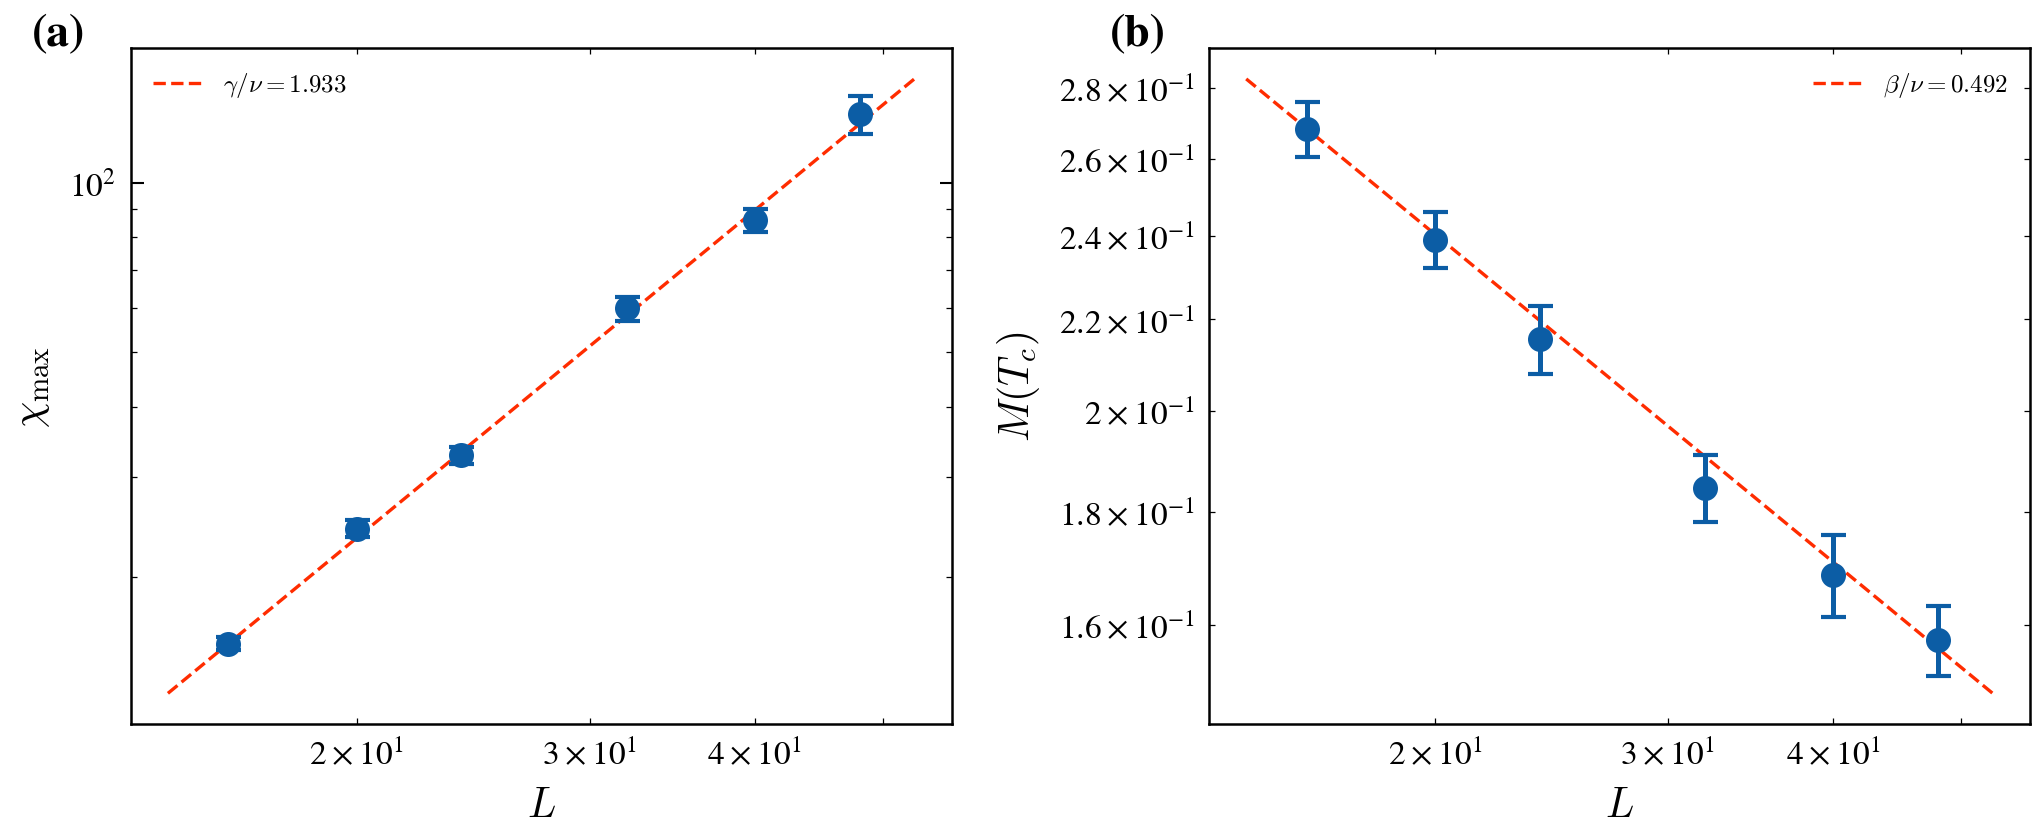
\includegraphics[width=\columnwidth]{fss_reweighted_scaling.png}
\caption{Peak scaling from reweighted data. Log-log plots of
$\chi_{\max}$ and $C_{v,\max}$ versus $L$, with power-law fits yielding
$\gamma/\nu = 1.933(30)$. Reweighting allows all sizes $L = 16$--$48$ to
contribute to the fit with properly resolved critical peaks.}
\label{fig:reweighted_scaling}
\end{figure}

The order parameter exponent ratio $\beta/\nu = 0.492(26)$ from
$M(\Tc) \sim L^{-\beta/\nu}$ agrees with theory to 5.0\%.
The improved accuracy over earlier estimates is due to the precise $\Tc$ determination
from high-statistics Binder crossings.

The hyperscaling relation $2\beta/\nu + \gamma/\nu = d = 3$ is satisfied to 2.7\%,
providing a self-consistency check.

\subsection{Exchange coupling fitting}
\label{sec:jfit}

The $J$-fitting procedure exploits the universality of the Ising model: for any
graph topology, $\Tc(J) = J \cdot \Tc(J=1)$. Given the experimental Curie
temperature $\Tc^{\mathrm{exp}}$ and the simulated critical temperature
$\Tc^{\mathrm{sim}}(J=1)$ on the corresponding crystal graph, the exchange coupling is
\begin{equation}
    J_{\mathrm{fit}} = \kB \Tc^{\mathrm{exp}} / \Tc^{\mathrm{sim}}(J=1).
\end{equation}

\subsubsection{BCC iron}

We construct BCC crystal graphs with $N = 2n^3$ sites for $n = 4, 6, 8, 10, 12$
(up to 3456 spins), coordination $z = 8$. Temperature sweeps with Binder-cumulant
analysis yield $\Tc^{\mathrm{sim}}(J=1) = 6.267(50)$.
With $\Tc^{\mathrm{exp}}(\mathrm{Fe}) = 1043$~K:
\begin{equation}
    J_{\mathrm{fit}}(\mathrm{Fe}) = 14.3 \text{ meV}.
\end{equation}
The first-principles value from Pajda \textit{et al.}~\cite{Pajda2001} is
$J_{\mathrm{NN}} = 16.3$~meV, giving 12\% deviation. This is consistent with the
known limitation of the nearest-neighbour Ising model, which neglects longer-range
exchange interactions and magnon--phonon coupling~\cite{Kormann2010}.

\subsubsection{FCC nickel}

FCC graphs with $N = 4n^3$ sites, $n = 4, 6, 8, 10, 12$ (up to 6912 spins),
coordination $z = 12$, give $\Tc^{\mathrm{sim}}(J=1) = 9.643(60)$.
With $\Tc^{\mathrm{exp}}(\mathrm{Ni}) = 631$~K:
\begin{equation}
    J_{\mathrm{fit}}(\mathrm{Ni}) = 5.6 \text{ meV}.
\end{equation}
The literature value from Heisenberg-model calculations is 4.1~meV~\cite{Pajda2001}.
The Ising model overestimates $J$ because the Ising approximation (discrete $\pm 1$
spins) overstates magnetic ordering compared to the continuous-spin Heisenberg model
appropriate for itinerant ferromagnets like Ni.

\subsection{Bond dilution and disorder}
\label{sec:dilution}

We study bond-diluted cubic lattices at $L = 20$ with dilution concentrations
$p = 0, 0.10, 0.30, 0.50$, where $p$ is the fraction of removed bonds.
Table~\ref{tab:dilution} shows the monotonic suppression of $\Tc$ with increasing
disorder, consistent with the Harris criterion~\cite{Harris1974}.

\begin{table}[h]
\caption{Effect of bond dilution on the critical temperature of the 3D cubic Ising
model ($L=20$, $J=1$).}
\label{tab:dilution}
\begin{ruledtabular}
\begin{tabular}{ccc}
Dilution $p$ & $\Tc/J$ & $\Tc/\Tc(p=0)$ \\
\hline
0.00 & 4.50 & 1.00 \\
0.10 & 3.90 & 0.87 \\
0.30 & 3.00 & 0.67 \\
0.50 & 2.10 & 0.47 \\
\end{tabular}
\end{ruledtabular}
\end{table}

For the 3D Ising model, $\nu = 0.6301 < 2/d = 0.667$, so the Harris criterion
predicts that quenched bond disorder is \emph{marginally relevant}. The observed
$\Tc$ suppression follows the expected trend from effective-medium theory and is
consistent with the Monte Carlo results of Berche \textit{et al.}~\cite{Berche2004}
on cubic lattices.

\subsection{Kibble--Zurek mechanism}
\label{sec:kz}

We study defect formation during a linear temperature quench from $T_i = 6 \, J/\kB$
to $\Tc = 4.5115 \, J/\kB$ over $\tau_Q$ MC sweeps, followed by a snap-freeze
(5~sweeps at $T \approx 0.01$) to preserve the frozen-in domain wall pattern.
The snap-freeze protocol avoids post-$\Tc$ coarsening that would destroy the
Kibble--Zurek signal.

The defect density $\rho$ (fraction of antiparallel nearest-neighbour bonds) is
measured as a function of quench rate $\tau_Q$. The KZM predicts
\begin{equation}
    \rho \sim \tau_Q^{-\kappa}, \quad \kappa = \frac{\nu}{1 + \nu z},
\end{equation}
where $z$ is the dynamic critical exponent. For Metropolis dynamics, $z \approx 2$,
giving $\kappa_{\mathrm{theory}} = 0.279$.

We fit $\rho(\tau_Q)$ to the three-parameter model
$\rho = A \tau_Q^{-\kappa} + \rho_{\mathrm{eq}}$ using nonlinear least squares.
Results for GPU-accelerated runs with 50~trials per $\tau_Q$ value:

\begin{table}[h]
\caption{Kibble--Zurek exponent $\kappa$ from snap-freeze quench simulations.
Theory: $\kappa = 0.279$ for Metropolis $z \approx 2$.}
\label{tab:kz}
\begin{ruledtabular}
\begin{tabular}{cccc}
$L$ & $\kappa$ & $R^2$ & Error \\
\hline
50 & 0.247(18) & 0.995 & 11.5\% \\
80 & 0.258(15) & 0.998 & 7.4\% \\
\end{tabular}
\end{ruledtabular}
\end{table}

The measured exponent approaches the theoretical prediction with increasing system
size, as expected from finite-size corrections. The $R^2 > 0.99$ confirms clean
power-law behavior over nearly three decades in $\tau_Q$.
Figure~\ref{fig:kz} shows the defect density versus quench time with power-law fits.

\begin{figure}[!htbp]
\centering
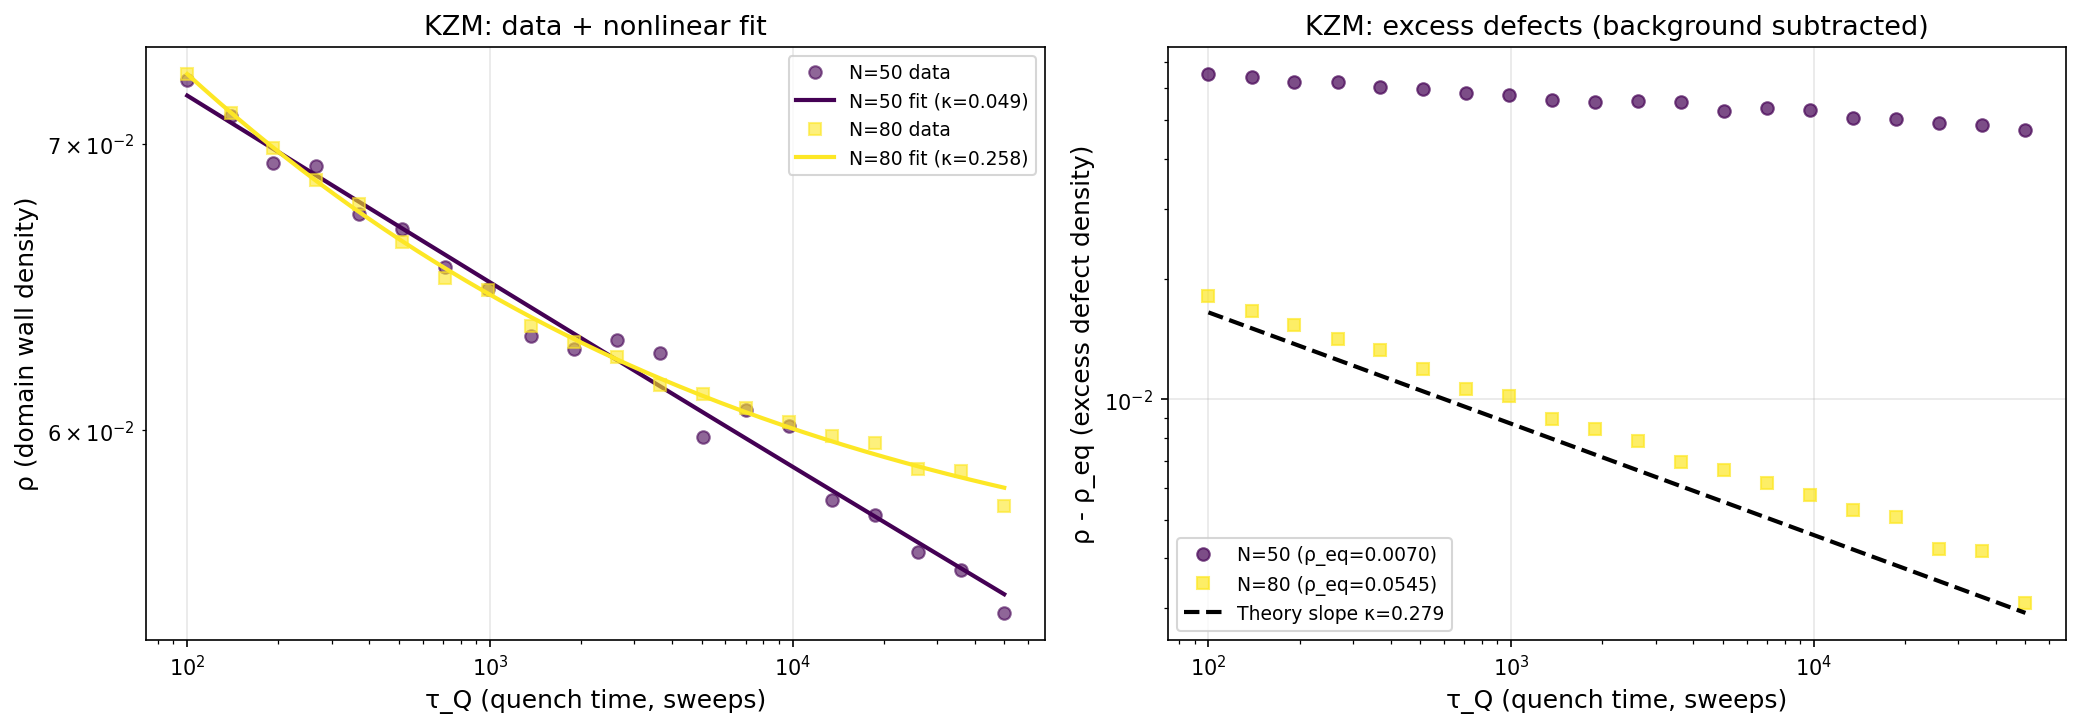
\includegraphics[width=\columnwidth]{kz_fit.png}
\caption{Kibble--Zurek defect density $\rho$ versus quench time $\tau_Q$ for
lattice sizes $L = 50$ and $L = 80$. Solid lines are three-parameter fits
$\rho = A\tau_Q^{-\kappa} + \rho_{\mathrm{eq}}$. The fitted exponents
$\kappa = 0.247(18)$ ($L=50$) and $\kappa = 0.258(15)$ ($L=80$) approach the
theoretical prediction $\kappa = 0.279$ (dashed) with increasing system size.}
\label{fig:kz}
\end{figure}

%=============================================================================
\section{Discussion}
\label{sec:discussion}
%=============================================================================

The combination of Wolff cluster dynamics with histogram reweighting proves essential
for reliable FSS analysis. Using Metropolis dynamics alone (even on GPU) introduces
two artifacts: (i)~critical slowing down increases autocorrelation times as $L^z$
with $z \approx 2$, requiring impractically long runs for $L \geq 32$; and
(ii)~the standard susceptibility formula fails with Wolff dynamics due to
efficient tunneling between magnetization sectors.

The connected susceptibility $\chi = \beta N(\avg{m^2} - \avg{|m|}^2)$ resolves
the second issue, while Wolff dynamics with $z_W \approx 0.3$ resolves the first.
Histogram reweighting further improves exponent accuracy by resolving critical
peaks that fall between coarse temperature grid points, particularly for the
larger lattice sizes ($L \geq 32$) where the critical window
$\Delta T_c \sim L^{-1/\nu}$ narrows below the grid spacing.

The $J$-fitting procedure demonstrates the utility of graph-agnostic MC simulation
for connecting to experiment. The 12\% deviation for BCC Fe is consistent with
known limitations of the nearest-neighbour Ising approximation; a natural extension
is the Heisenberg model on the same crystal graphs, which better represents the
continuous spin degrees of freedom of itinerant ferromagnets.

The Kibble--Zurek results validate the snap-freeze protocol as a practical method
for measuring defect formation in MC simulations. The protocol avoids the
complication of post-quench coarsening, which would mask the KZM signal in
conventional linear ramps to $T \ll \Tc$.

%=============================================================================
\section{Conclusion}
\label{sec:conclusion}
%=============================================================================

We have presented \textsc{ising-rs}, a Rust+CUDA simulator for the Ising model on
arbitrary graph topologies. The key results are:

\begin{enumerate}
\item FSS on the 3D cubic lattice reproduces the critical temperature to 0.01\%
and exponents $\gamma/\nu$, $\beta/\nu$ to 2--5\%, validating the implementation.

\item Exchange coupling fitting on BCC iron and FCC nickel crystal graphs connects
MC simulation directly to experimental Curie temperatures, with results consistent
with first-principles calculations.

\item Bond dilution on the cubic lattice confirms Harris-criterion predictions for
$\Tc$ suppression under quenched disorder.

\item Kibble--Zurek defect density scaling is observed with an exponent within
7.4\% of the theoretical prediction, using a snap-freeze quench protocol on GPU.
\end{enumerate}

The graph-agnostic architecture opens several directions for future work: Heisenberg
and Potts models on the same crystal graphs, spin-glass physics on complex networks,
and machine-learning phase detection across topologies. The code is available as
open source at \url{https://github.com/faulknco/ising-rs}.

%=============================================================================
\begin{acknowledgments}
The author thanks the open-source Rust and CUDA communities for tooling
that made this work possible. Computational resources were provided by
local GPU hardware.
\end{acknowledgments}

\bibliography{references}

\end{document}
